\chapter{Lepton (electron) Scattering}
    \section{Overview}
        We can probe the structure of sub-atomic particles by shooting high energy particles at them. The higher the energy, the shorter distances we resolve. This was done for example in the early 1900s with Rutherford scattering, leading to the discovery of the nucleus in the atom.\\
        \indent For probing the structure of the proton, ideal scattering particles are leptons, as they are point particles with (apparently) no sub-structure themselves. Electrons are the simplest to use as they are stable and easy to produce, but muons and neutrinos are also used.\\
        \indent A key concept is that increasing the energy of the incident particle allows you to resolve shorter distances, which corresponds to different scattering cross sections as you change energy. The following plot illustrates this and is essential:\\
    
        \begin{figure}[H]
            \centering
            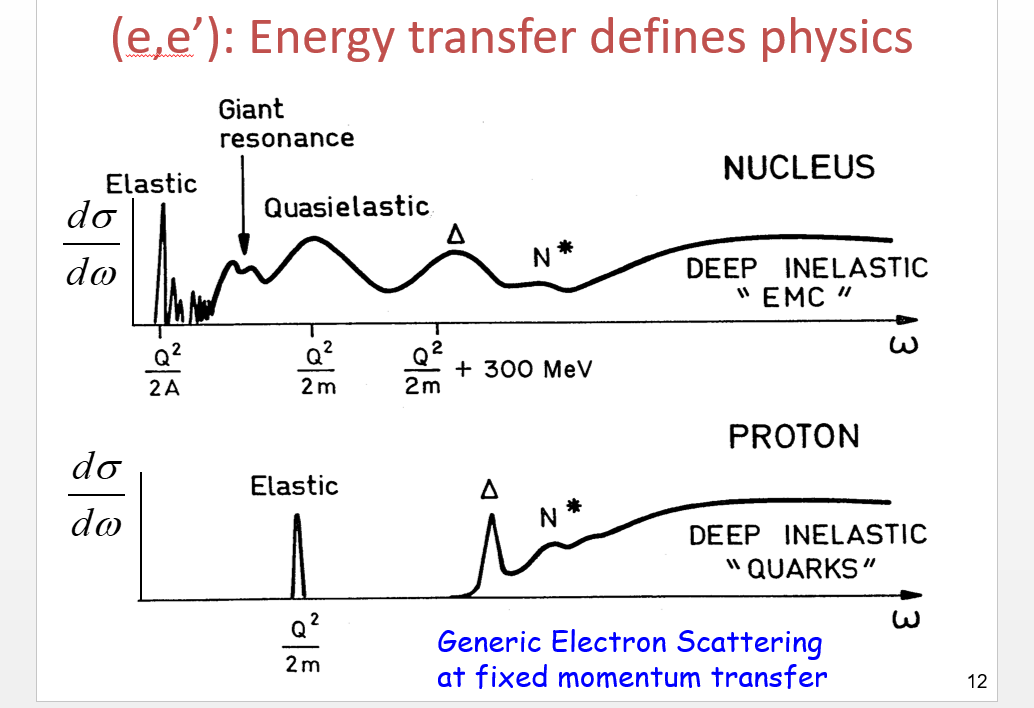
\includegraphics[width=10cm]{NuclearPhysics/modules/lepton-scattering/pics/e-p-scattering.png}
            \caption{Electron-proton scattering cross section vs. energy transfer $\omega$}
        \end{figure}
    \section{Quasi-Elastic}
        Quasielastic – is broadened due to fermi motion, also slightly shifted due to binding energy of nucleon in nucleus.
\chapter{Elastic Scattering}

    \section{Elastic Low Energy (Proton = Point) Limit: Rutherford and Mott Scattering}
        \indent Both Rutherford and Mott scattering neglect the proton recoil and treat the proton as a point source. \\
        \indent The Feynman calculations for this process are straightforward and carried through exactly in Thomson 7.2. \\
        
        \begin{figure}[H]
            \centering
            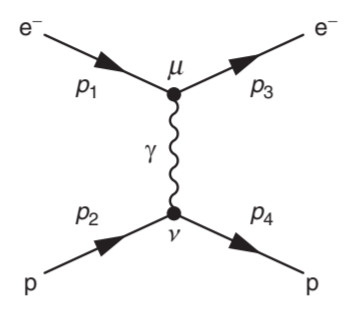
\includegraphics[width=10cm]{NuclearPhysics/modules/lepton-scattering/pics/elastic-ep/rut-1.PNG}
            \caption{Diagram for basic ep scattering}
        \end{figure}
        
        \begin{figure}[H]
            \centering
            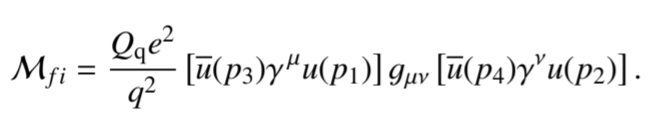
\includegraphics[width=8cm]{NuclearPhysics/modules/lepton-scattering/pics/elastic-ep/rut-matrix.PNG}
            \caption{Matrix element for ep scattering}
        \end{figure}
        
        \begin{figure}[H]
            \centering
            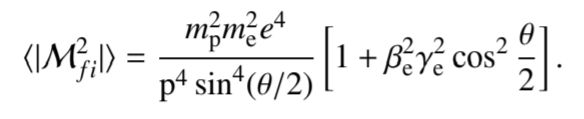
\includegraphics[width=6cm]{NuclearPhysics/modules/lepton-scattering/pics/elastic-ep/full-matrix.PNG}
            \caption{Result of matrix element calculation}
        \end{figure}
        
        \subsection{Rutherford scattering}
            \indent Rutherford scattering assumes the electron is non-relativistic, yielding a cross section of:

                \begin{equation}
                    \frac{d\sigma}{d\Omega} = \frac{\alpha^2}{16E^2_K\sin^4{(\theta/2)}}
                \end{equation}
                %\myequations{Rutherford Scattering}
            
            In this non-relativistic limit, only the interaction between the electric charges of the electron and proton contribute; there is no magnetic (spin-spin) interaction. The angular dependence originates only from the 1/$q^2$ propagator term.
            
        \subsection{Mott Scattering}
            \indent Mott scattering has a relativistic electron but still fixed point proton. Now since electron momentum is about equal to its energy, reductions lead to the Mott cross section:
            
                \begin{equation}
                    \frac{d\sigma}{d\Omega} = \frac{\alpha^2}{4E^2\sin^4{(\theta/2)}}\cos^2{\frac{\theta}{2}} = \left( \frac{\alpha}{2E\sin^2{(\theta/2)}}\cos{\frac{\theta}{2}} \right)^2
                \end{equation}
                %\myequations{Mott Scattering}
            
            Again, purely magnetic spin-spin interactions are negligible here. 
            
        \subsection{Summary}
            Rutherford - elastic scattering, proton = fixed, point, electron $\neq$ relativistic\\
            Mott - elastic scattering, proton = fixed, point, electron = relativistic
        
            \begin{equation}
                (\frac{d\sigma}{d\Omega})_{Mott} = 4\cos^2{\frac{\theta}{2}}(\frac{d\sigma}{d\Omega})_{Ruth}
            \end{equation}
    \section{Form Factors: Accounting for Proton Structure}
        \indent If the proton were a point, then the Mott Scattering cross section would agree with experiment for all electron scattering energies. Instead, deviations from Mott are observed as we increase the beam energy. To account for this structure, we need to define form factors, which describe the structure of the proton:
        
        \begin{equation}
            \frac{d\sigma}{d\Omega} = \frac{\alpha^2}{4E^2\sin^4{(\theta/2)}}\cos^2{\frac{\theta}{2}}(F(\textbf{q}^2))^2
        \end{equation}
        
        
        $F(\textbf{q}^2)$ is the 3D Fourier transform of the charge distribution: 
        
        \begin{figure}[H]
            \centering
            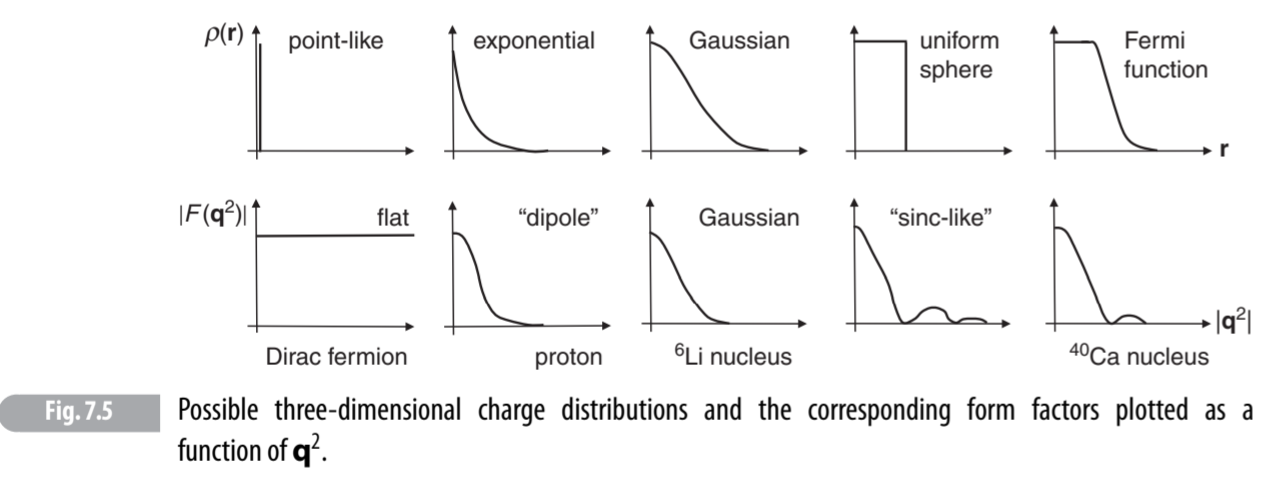
\includegraphics[width=14cm]{NuclearPhysics/modules/lepton-scattering/pics/elastic-ep/charge-dist.PNG}
            \caption{Charge Distribution Fourier Transforms}
        \end{figure}
        
        In general, a spin S particle will have 2S + 1 form factors. For example, a proton is spin 1/2, and has 2 form factors. A spin 3/2 particle will have 4 form factor (e.g. Li7) 
        
    \section{Relativistic Electron Proton Elastic Scattering}
        \indent Explicit math is worked out in Thomson 7.4 and is straightforward, but important relations are:
        
        \begin{figure}[H]
            \centering
            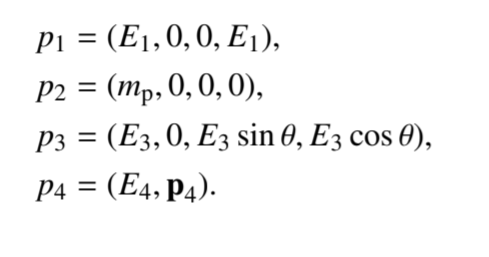
\includegraphics[width=6cm]{NuclearPhysics/modules/lepton-scattering/pics/elastic-ep/kine-e-1.PNG}
            \caption{Kinematic 4-vectors of particle momentum}
        \end{figure}
        
        \begin{figure}[H]
            \centering
            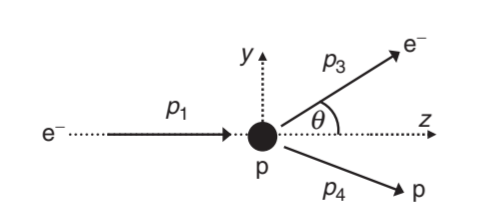
\includegraphics[width=10cm]{NuclearPhysics/modules/lepton-scattering/pics/elastic-ep/kine-e-2.PNG}
            \caption{Elastic scattering diagram}
        \end{figure}
        
        From the electron - photon - electron vertex, we get the four-momentum squared of the virtual photon (neglect the mass of the electron) $q^2$:
        
        \begin{equation}
            Q^2 = -q^2 = 4E_1E_3\sin^2(\frac{\theta}{2})
        \end{equation}
        
         We can $E_3$ expressed in terms of the scattering angle of the electron:
         
        \begin{equation}
            E_3 = \frac{E_1m_p}{m_p+E_1(1-\cos\theta)}
        \end{equation}
        
        This lets us rewrite $Q^2$ as:
        
        \begin{equation}
            Q^2 = \frac{2m_pE_1^2(1-\cos\theta}{m_p+E_1(1-\cos\theta)}\label{eq:2}
        \end{equation}
        %\myequations{$Q^2$ - Incident Electron Energy Relation, Elastic Scattering}
        
        Which gives us the differential cross section for the scattering of relativistic electrons from a pointlike proton as: 
        
        \begin{equation}
            \frac{d\sigma}{d\Omega} = \frac{\alpha^2}{4E_1^2\sin^4{(\theta/2)}}\frac{E_3}{E_1}(\cos^2{\frac{\theta}{2}}+\frac{Q^2}{2m_p^2}\sin^2(\frac{\theta}{2}))
        \end{equation}
       % \myequations{Elastic Scattering Cross Section - pointlike proton}
        
        \subsection{Important Notes}
            \indent Elastic ep scattering has only 1 independent variable, so measuring the scattering angle determines all of the kinematics. In practice, by measuring the energy and angle of scattered electrons, the system can be over constrained to ensure that the scattering was in fact elastic. \\

            \indent Compared to Mott Scattering, there are two differences in the elastic scattering formula. The $E_3/E_1$ term in the scattering cross section comes from the electron losing energy to the proton's final state kinetic energy (no longer a fixed source). The new term proportional to $\sin^2(\theta/2)$ is due to a purely magnetic spin-spin interaction. 
    \section{Rosenbluth}
        \indent The derived cross-section for elastic scattering still lacks any proton structure. To incorporate structure, we need to include two form factors, $G_E(Q^2)$ - related to the distribution of charge, and $G_M(Q^2)$, related to the distribution of the magnetic moment inside the proton. In the low-$Q^2$ limit, these form factors are the Fourier transforms of the charge an magnetic moment distributions, but the carryover is not exact in general due to being functions of the 4-momenta, instead of 3 momenta. E.g.:
        
        \begin{figure}[H]
            \centering
            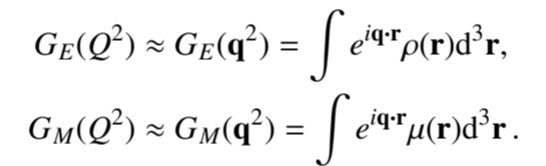
\includegraphics[width=6cm]{NuclearPhysics/modules/lepton-scattering/pics/elastic-ep/fourier-gegm.PNG}
            \caption{Interpretations of $G_E$ and $G_M$}
        \end{figure}
        
        Including these form factors in our cross section gives us the full elastic scattering cross section:
                
        \begin{equation}
            \frac{d\sigma}{d\Omega} = \frac{\alpha^2}{4E_1^2\sin^4{(\theta/2)}}\frac{E_3}{E_1}\left( \frac{G_E^2+\tau G_M^2}{1+\tau} \cos^2{\frac{\theta}{2}}+2\tau G_M^2\frac{Q^2}{2m_p^2}\sin^2(\frac{\theta}{2})\right)
        \end{equation}
       % \myequations{Full Elastic Scattering Cross Section}
        
        Here $\tau$ is:
                
        \begin{equation}
            \tau = \frac{Q^2}{4m_p^2}
        \end{equation}
        
        
        \subsection{Rosenbluth Separation - Measuring Ge and Gm}
            \indent By increasing our beam energy, we will see deviations away from Mott scattering behaviour. We see this explicitly by rewriting the scattering formula as:
            
            \begin{equation}
                \frac{d\sigma}{d\Omega} = \left( \frac{G_E^2+\tau G_M^2}{1+\tau} +2\tau G_M^2\tan^2(\frac{\theta}{2})\right) \left( \frac{d\sigma}{d\Omega}_0\right)
            \end{equation}
      %  \myequations{Full Elastic Scattering Cross Section}
        
        
        Where $\frac{d\sigma}{d\Omega}_0$ is the Mott Scattering cross section, with the factor of $\frac{E_3}{E_1}$ included to account for proton recoil. We can then extract $G_E$ and $G_M$ in the following way (\textbf{"Rosenbluth Separation"}):\\
        \subsection{Rosenbluth Method Walk through}
            \subsubsection{Take Data}
                1.) Experimental set up - electron beam scattering off of proton target. Could use something like GaAs source, Linac up to 0.1 - 1 GeV, incident on proton target, liquid hydrogen should be fine. For a detector, use a dipole spectrometer with scintillating tile focal plane, or something else to measure position well (MWPC, (cheap) silicon strips (expensive, good resolution)). You want to measure the electrons energy so you know $E_3$, e.g. you want to be able to over constrain the event so you know it was in fact elastic. Other than that you are just counting events.\\
                
                2.) Put spectrometer at 135 degrees in theta from the beam axis. Take data at 10 different beam energies. You know know the cross section at that angle at that energy. Now move the spectrometer to 120 degrees. Repeat energy scan. Repeat this process for several other beam angles. You are done taking data.
            \subsubsection{Analyze data}
                1.) Go into your data. Using the relation between $Q^2$, $\theta$, and $E_1$, pick a value of $Q^2$ (e.g. 0.292 GeV$^2$, invert to find the beam energy at the appropriate $\theta$, and note the cross section at that point. What you just did is find the cross-section value at that angle, corresponding to a specific $Q^2$ value. Repeat for all the angles you had your spectrometer at. You now have a plot of cross section vs. angle ($\tan(\theta^2)$ so that it is a line), at a specific $Q^2$ value. \\
                2.) Now fit a line to the data. The slope gives you $G_M$ at that $Q^2$, and the y-intercept gives you $G_E$ at that $Q^2$ (see \label{eq:1})\\
                3.) Repeat steps 1 and 2 for as big of a $Q^2$ range that you can. \\
                \newline
                Side notes from Axel - the Rosenbluth method has awful systematics - need to measure absolute cross sections, radiative corrections become large, uncertainties for $G_E$ and $G_M$ are correlated, etc.
            \subsubsection{Results}
                Carrying out this procedure gives you plots of $G_E$ and $G_M$ vs. $Q^2$. 
                
                We see as $Q^2$ goes to zero, we recover $G_E$ = 1 and $G_M$ = 2.79, as it should. The data fits well to the so called "dipole function" i.e.:
                \begin{figure}[H]
                    \centering
                    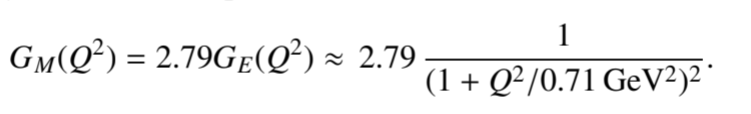
\includegraphics[width=8cm]{NuclearPhysics/modules/lepton-scattering/pics/elastic-ep/dipole.PNG}
                    \caption{Rosenbluth Results}
                \end{figure}
                This relates to a proton charge distribution as exponentially falling off, i.e.\\
                $\rho(r) \sim \rho_0 e^{-r/a}$\\
                Here a = 0.24 fm, which corresponds to a proton RMS charge radius of 0.8 fm. \\
                Finally, at high $Q^2$, $G_M \propto Q^{-4}$, which means that the elastic scattering cross section falls as $1/Q^6$
                Also, we can calculate the RMS charge radius of the proton as:
                
             
                \begin{figure}[H]
                    \centering
                    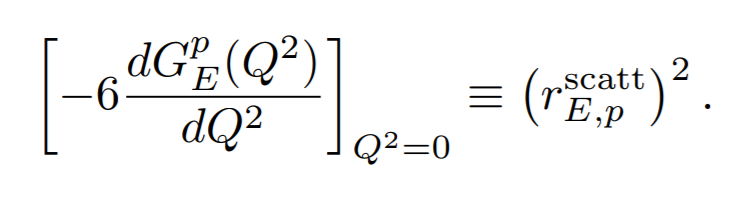
\includegraphics[width=6cm]{NuclearPhysics/modules/emc-src-scaling/pics/prad-GE.PNG}
                \caption{Taylor expansion of $G_E$ to yield proton charge radius}
                \end{figure}
    \section{Olympus and TPEX}
        The Rosenbluth method of measuring the ratio of $G_E$ and $G_M$ has awful systematics, based mainly in the facts that you need to measure an absolute cross section, worry about radiative corrections, and measure at low $Q^2$. A better way to measure the proton form factor ratio is by a \textbf{polarization transfer} measurement. This uses a \textbf{Focal Plane Polarimeter} to converst transverse polarization into an azimuthal distribution:
        
              
        \begin{figure}[H]
            \centering
            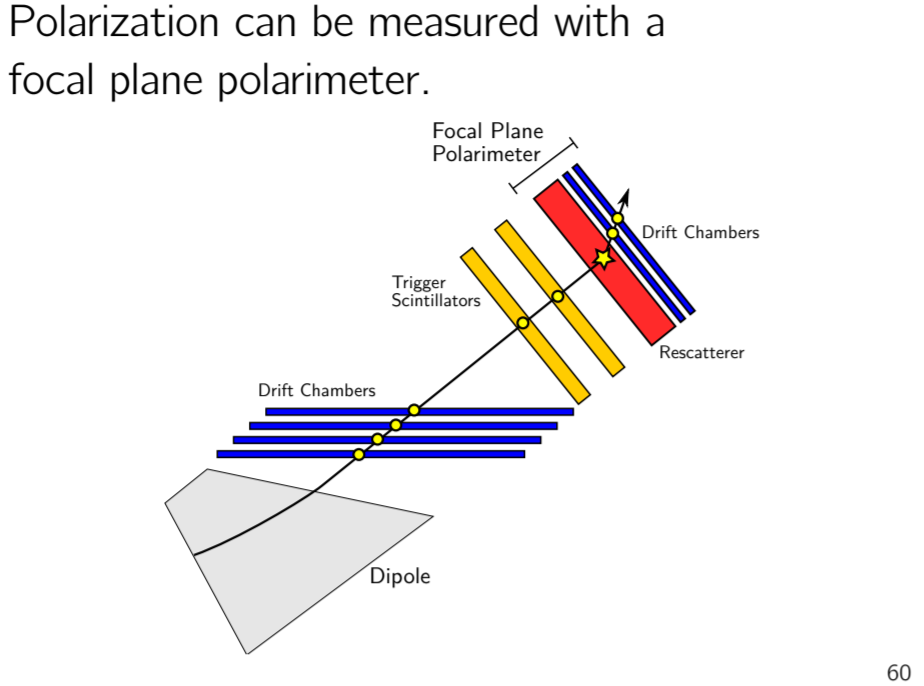
\includegraphics[width=10cm]{NuclearPhysics/modules/lepton-scattering/pics/elastic-ep/olympus-fpp.PNG}
            \caption{Olympus experimental setup}
        \end{figure}
        
        This method has the advantages that we are measuring a ratio, not an absolute cross section, so many uncertainties cancel, such as the FPP analyzing power. Olympus produced the following:
        
              
        \begin{figure}[H]
            \centering
            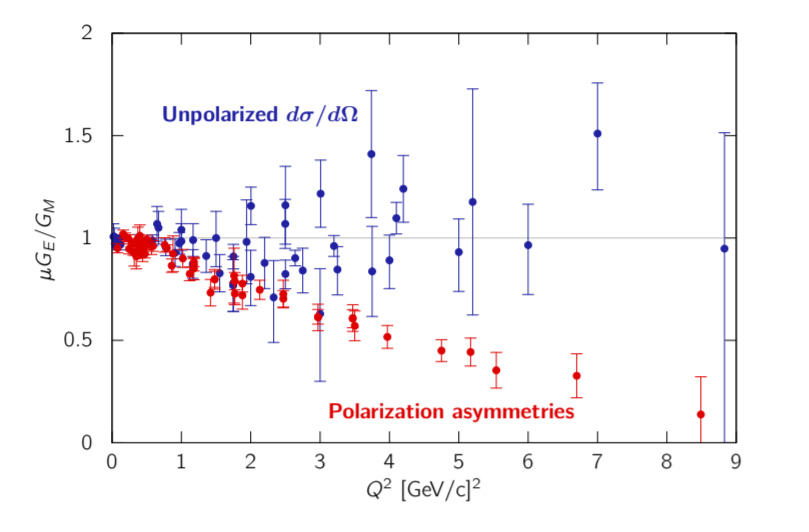
\includegraphics[width=10cm]{NuclearPhysics/modules/lepton-scattering/pics/elastic-ep/olympus-form-factors.PNG}
            \caption{$G_E$ and $G_M$ ratio measurements}
        \end{figure}
        
        This discrepancy may be due to two photon exchange, which we can measure by comparing electron to positron scattering:
        
              
        \begin{figure}[H]
            \centering
            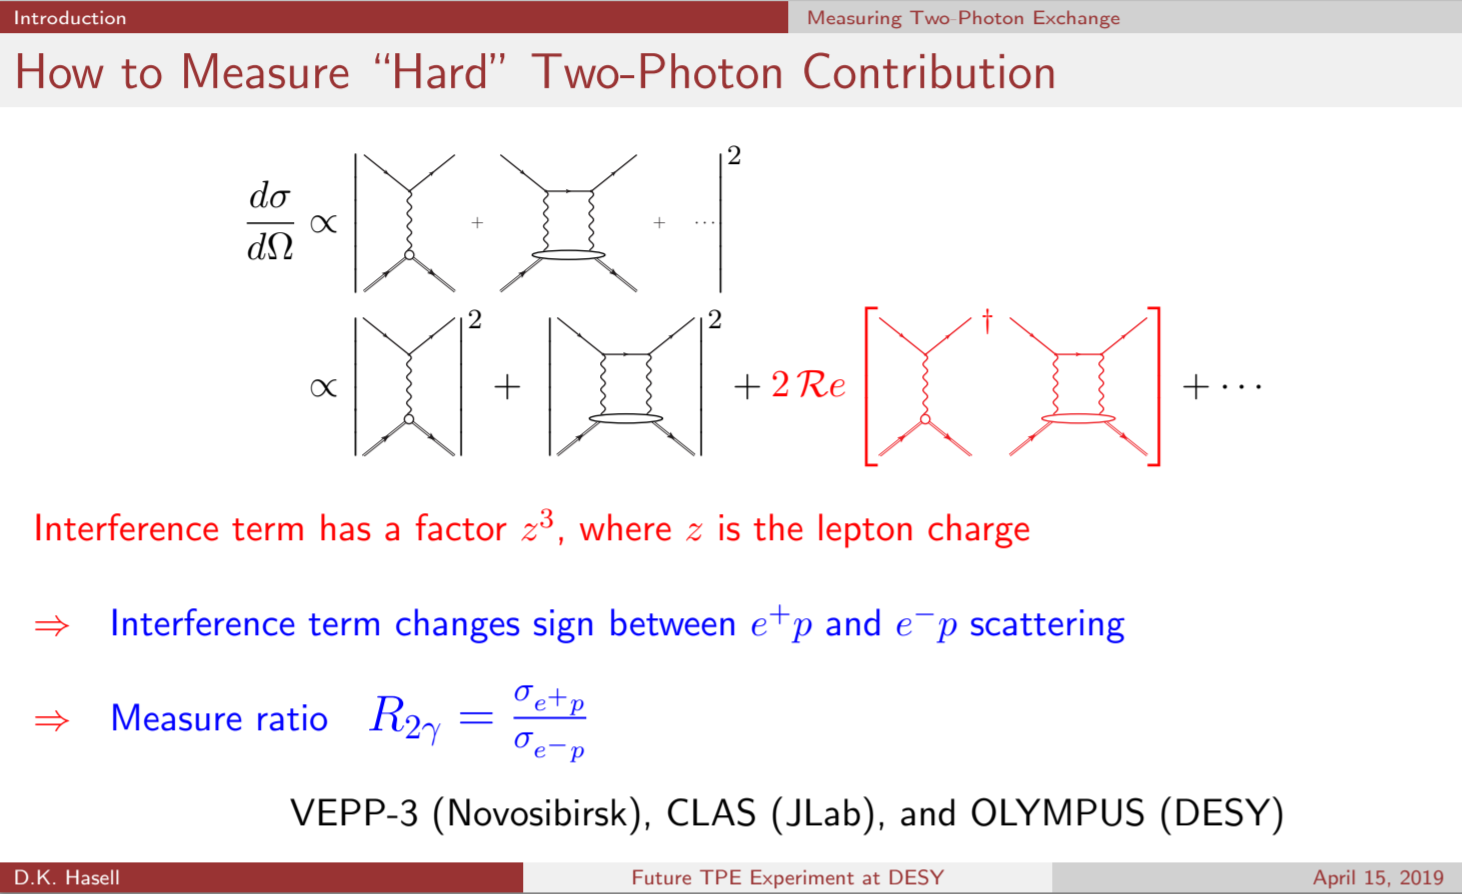
\includegraphics[width=10cm]{NuclearPhysics/modules/lepton-scattering/pics/elastic-ep/tpex.PNG}
            \caption{Electron Positron charge interference}
        \end{figure}
    
    
        TPEX is a currently proposed experiment to extend this out to farther $Q^2$, which is challenging due to its lower luminosity of elastic scattering as $Q^2$ increases.     
       
\chapter{Inelastic Scattering}
    \section{Overview}
        In inelastic scattering, we now no longer require that the proton remains intact, and we can create resonances, or as we increase the energy, can create a slew of hadronic final states. Since we remove the constraint that the mass of the final state is the proton mass, we now have one extra degree of freedom, i.e., we need 2 variables to describe inelastic scattering. These are usually Bjorken X $x_B$ and the 4-momentum transfer of the virtual photon $Q^2$.\\
        N.B. - 1990 Nobel Prize awarded to Friedman, Kendall, and Taylor "for their pioneering investigations concerning deep inelastic scattering of electrons on protons and bound neutrons, which have been of essential importance for the development of the quark model in particle physics"
    \section{Variables}
                
        \subsection{Bjorken X}
        Think of Xb as the ratio of momentum transfer to energy transfer. 
        
        $x_B$ is a measure of elasticity - 1 for elastic scattering. Also, is the fraction of proton momentum carried by the struck quark in the infinite momentum frame.
        \begin{equation}
            x = \frac{Q^2}{2p_2\cdot q} = \frac{Q^2}{Q^2+W^2-m_p^2}
        \end{equation}
        %\myequations{Bjorken X}
    
            Derivation of infinite momentum frame Bjorken x. Take quark to have momentum fraction $\xi$ of proton's total momentum,i.e. $p_q = \xi p_2$:\\
            \indent Inf. Mom. frame - neglect proton mass so $p_2$ = $E_2$, neglect all transverse momenta:\\
            \indent Struck quark 4-momenta: $p_q = \xi p_2 = (\xi E_2, \xi E_2, 0, 0)$\\
            \indent 4-momenta of quark after interaction: $(p_q + q) = (\xi p_2 +q)$\\
            \indent Square the 4-momenta $(\xi p_2 +q)^2 = \xi^2 p_2^2 +q^2 + 2\xi p_2 \cdot q  = m_q^2$\\
            \indent Continue, noting $p_q = \xi p_2$ : $m_q^2 = p_q^2 - Q^2 + 2 \xi p_2 \cdot q$\\
            \indent Since $p_q^2$ = $m_q^2$, we have: $m_q^2 = m_q^2 -Q^2 + 2 \xi p_2 \cdot q$\\
            \indent So $0 = -Q^2 + 2\xi p_2 \cdot q \longrightarrow \xi = \frac{Q^2}{2 p_2 \cdot q} = x_B$\\
        
        
        \subsection{Y}
        y is a measure of the inelasticity of the scattering, it is the fractional energy lost by the electron in the scattering process (second equality is true where proton is at rest). 0 is for perfectly elastic, 1 is for entirely inelastic. 
        
        \begin{equation}
            y = \frac{p_2 \cdot q}{p_2 \cdot p_1} = 1 - \frac{E_3}{E_1}
        \end{equation}
        
        \subsection{Q2}
        With these variables, we can make the equality for $Q^2$:
        
          \begin{equation}
            Q^2 = (s-m_p^2)xy \sim sxy
        \end{equation}
        
        Since you are now breaking up the proton, you have an additional degree of freedom, so you need two observables to describe inelastic scattering. 
        

        \subsection{W}
            W is the four momenta of the final state system that started with the proton, W = q + $p_2$. It is useful as $W^2 = m_p^2 -Q^2 + 2 p_2 \cdot q$
        
    \section{Deep Inelastic Scattering}
        \indent To describe further proton sub-structure, we need to introduce structure functions, $F_1(x,Q^2)$ - purely magnetic, and $F_2(x,Q^2)$. For DIS where $Q^2 >> m_p^2y^2$, we have the following cross section formula:
        
        \begin{figure}[H]
            \centering
            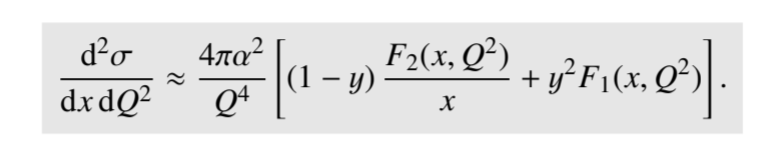
\includegraphics[width=10cm]{NuclearPhysics/modules/lepton-scattering/pics/inelastic-ep/dis-xsection.PNG}
            \caption{General DIS cross section}
        \end{figure}
    \section{Bjorken Scaling and Callan Gross}
        \indent In DIS, we observe Bjorken scaling and Callan-Gross
        
        \begin{figure}[H]
            \centering
            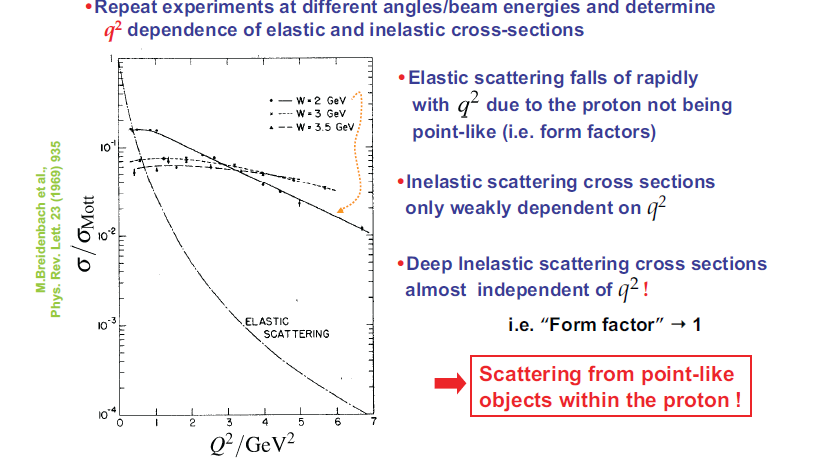
\includegraphics[width=10cm]{NuclearPhysics/modules/lepton-scattering/pics/inelastic-ep/DIS.png}
            \caption{Early Bjorken Scaling Example}
        \end{figure}
        
        After performing DIS measurements at SLAC with electron energies between 5 and 20 GeV on liquid hydrogen, using a movable spectrometer over various angles, showed two important results:\\
        \newline
        \textbf{Bjorken Scaling} where $F_1$ and $F_2$ are basically flat with respect to $Q^2$, and thus are independent of $Q^2$, indicating that we are scattering off point-like constituents inside the proton.\\
        \newline
        \textbf{Callan Gross Relation} where $F_2 = 2x F_1$, a relation which can be explained by assuming the underlying process is actually elastic scattering off of point-like spin-half constituents inside the prton (quarks). 
    \section{Structure Functions and Parton Distribution Functions}
        \indent These describe the distribution of quarks within the nucleon. Describes the momentum fraction distribution of quarks. For example:\\
        \newline
        $u^p(x)dx$\\
        \newline
        Represents the number of up-quarks within the proton with momentum fraction between x and dx. The functional forms of the PDFs are not a-priori known. Some potential PDFs could be as shown below:\\
        
        \begin{figure}[H]
            \centering
            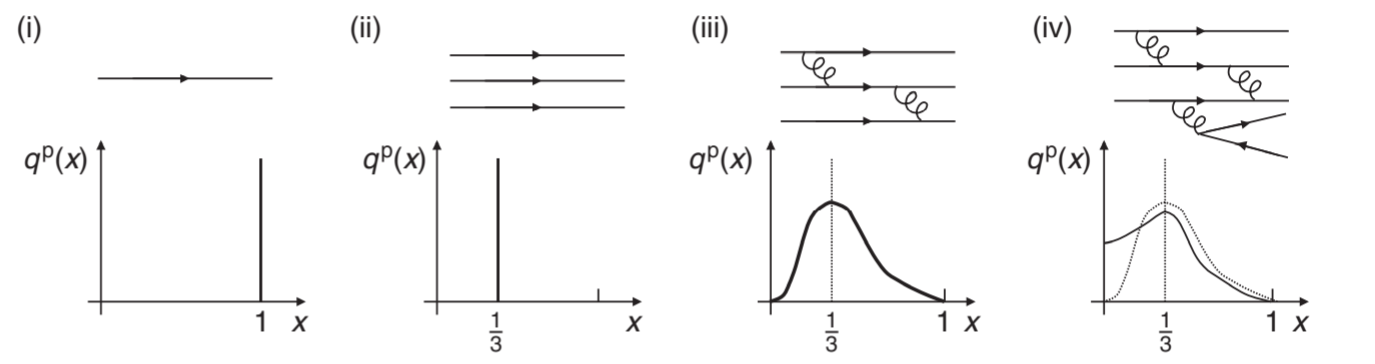
\includegraphics[width=12cm]{NuclearPhysics/modules/lepton-scattering/pics/inelastic-ep/pdf-possibilities.PNG}
            \caption{Potentail PDFs}
        \end{figure}
        
        (i) - if the proton consisted of a single quark\\
        (ii) - if the proton had 3 static quarks\\
        (iii) - quarks interacting and Heisenberg uncertainty (momentum smearing)\\
        (iv) - interacting quarks with higher order diagrams - gluons produced, so enhances low x part of PDF\\
        \newline
        We can access these distributions experimentally as the parton model predicts the the cross section for elastic scattering off of quarks with charge $Q_i$ and momentum fraction in the range of x to x + dx as:
        
               
        \begin{figure}[H]
            \centering
            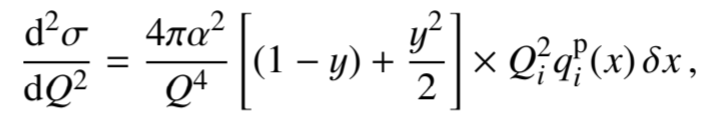
\includegraphics[width=8cm]{NuclearPhysics/modules/lepton-scattering/pics/inelastic-ep/quark-x.PNG}
            \caption{Quark scattering cross section}
        \end{figure}
        
        So then the cross section summing over all quark flavours is:
        
               
        \begin{figure}[H]
            \centering
            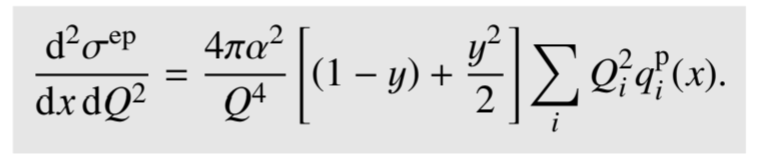
\includegraphics[width=8cm]{NuclearPhysics/modules/lepton-scattering/pics/inelastic-ep/quark-x-sum.PNG}
            \caption{Quark PDF - cross section relation}
        \end{figure}
        
        and comparing it with the general expression for DIS cross section:
        
                
        \begin{figure}[H]
            \centering
            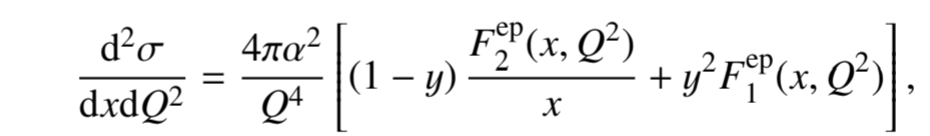
\includegraphics[width=8cm]{NuclearPhysics/modules/lepton-scattering/pics/inelastic-ep/inel-general.PNG}
            \caption{General DIS cross section}
        \end{figure}
        We see we can get the relation:
        
                
        \begin{figure}[H]
            \centering
            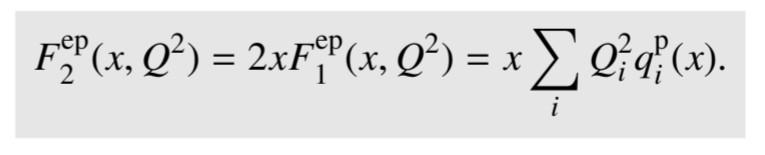
\includegraphics[width=8cm]{NuclearPhysics/modules/lepton-scattering/pics/inelastic-ep/f2-sum-q.PNG}
            \caption{Structure function - quark PDF relatio}
        \end{figure}
        
        For an explicit example, we have (neglecting heavier quarks, which have smaller contributions):
        
                
        \begin{figure}[H]
            \centering
            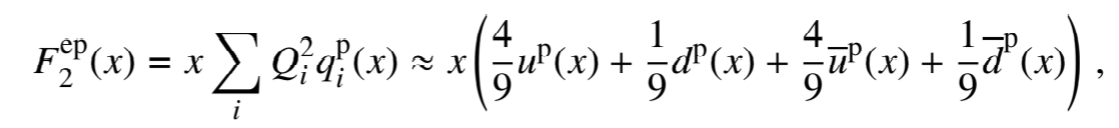
\includegraphics[width=12cm]{NuclearPhysics/modules/lepton-scattering/pics/inelastic-ep/example-f2.PNG}
            \caption{Up and Down quark contributions to structure functions}
        \end{figure}
        
        Note that the parton model predicts both Bjorken scaling and the Callan Gross relation. Importantly, because QCD is hard, the PDFs cannot be calculated from perterbation theroy, and must be measured in DIS. We can integrate the PDFs to determine the total momentum fraction of the proton carried by each flavour of quark, as:
        
                
        \begin{figure}[H]
            \centering
            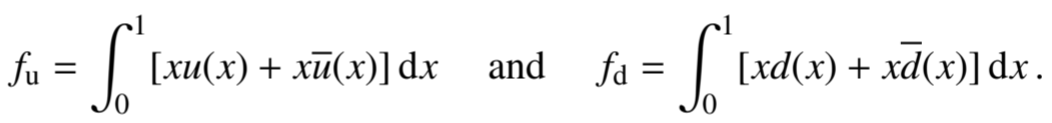
\includegraphics[width=12cm]{NuclearPhysics/modules/lepton-scattering/pics/inelastic-ep/integrated-ud.PNG}
            \caption{Total quark momentum fractions}
        \end{figure}
        
        Doing this after DIS measurements yields $f_u = 0.36$ and $f_d = 0.18$, so the u and d quarks only carry about half of the total momentum of the proton. The rest is carried by gluons, which do not interact in QED ep scattering. \\
        
        There are other predictions to be made here, such as the ratio of $F_2$ in neutrons vs. in protons. It would be expected that the ratio would go to 1 as $x_B$ goes to 0, as at low x the PDF is dominated by sea quarks and gluons, which are independent of nucleon type. At high $Q^2$ we would expect some ratio as basically the number f up quarks to down quarks, but this is not what is seen; instead we observe a modification which might be explained by the fact that it is more likely to have one up quark at high momentum, as if the one down quark were at high momentum, the two up quarks would be closer in phase space, which is disfavoured by the Pauli Exclusion principle. 
    \section{Scaling and Violations}
        Structure functions were studied in great detail (one million DIS events at $Q^2$ greater than 200 GeV$^2$ - kinematic range was up to $Q^2 = 20,000 GeV^2$ and $x < 0.0001$. $Q^2$ and $x$ were determined solely by precisely measuring the scattering angle and energy of the electron. 
        
        \begin{figure}[H]
            \centering
            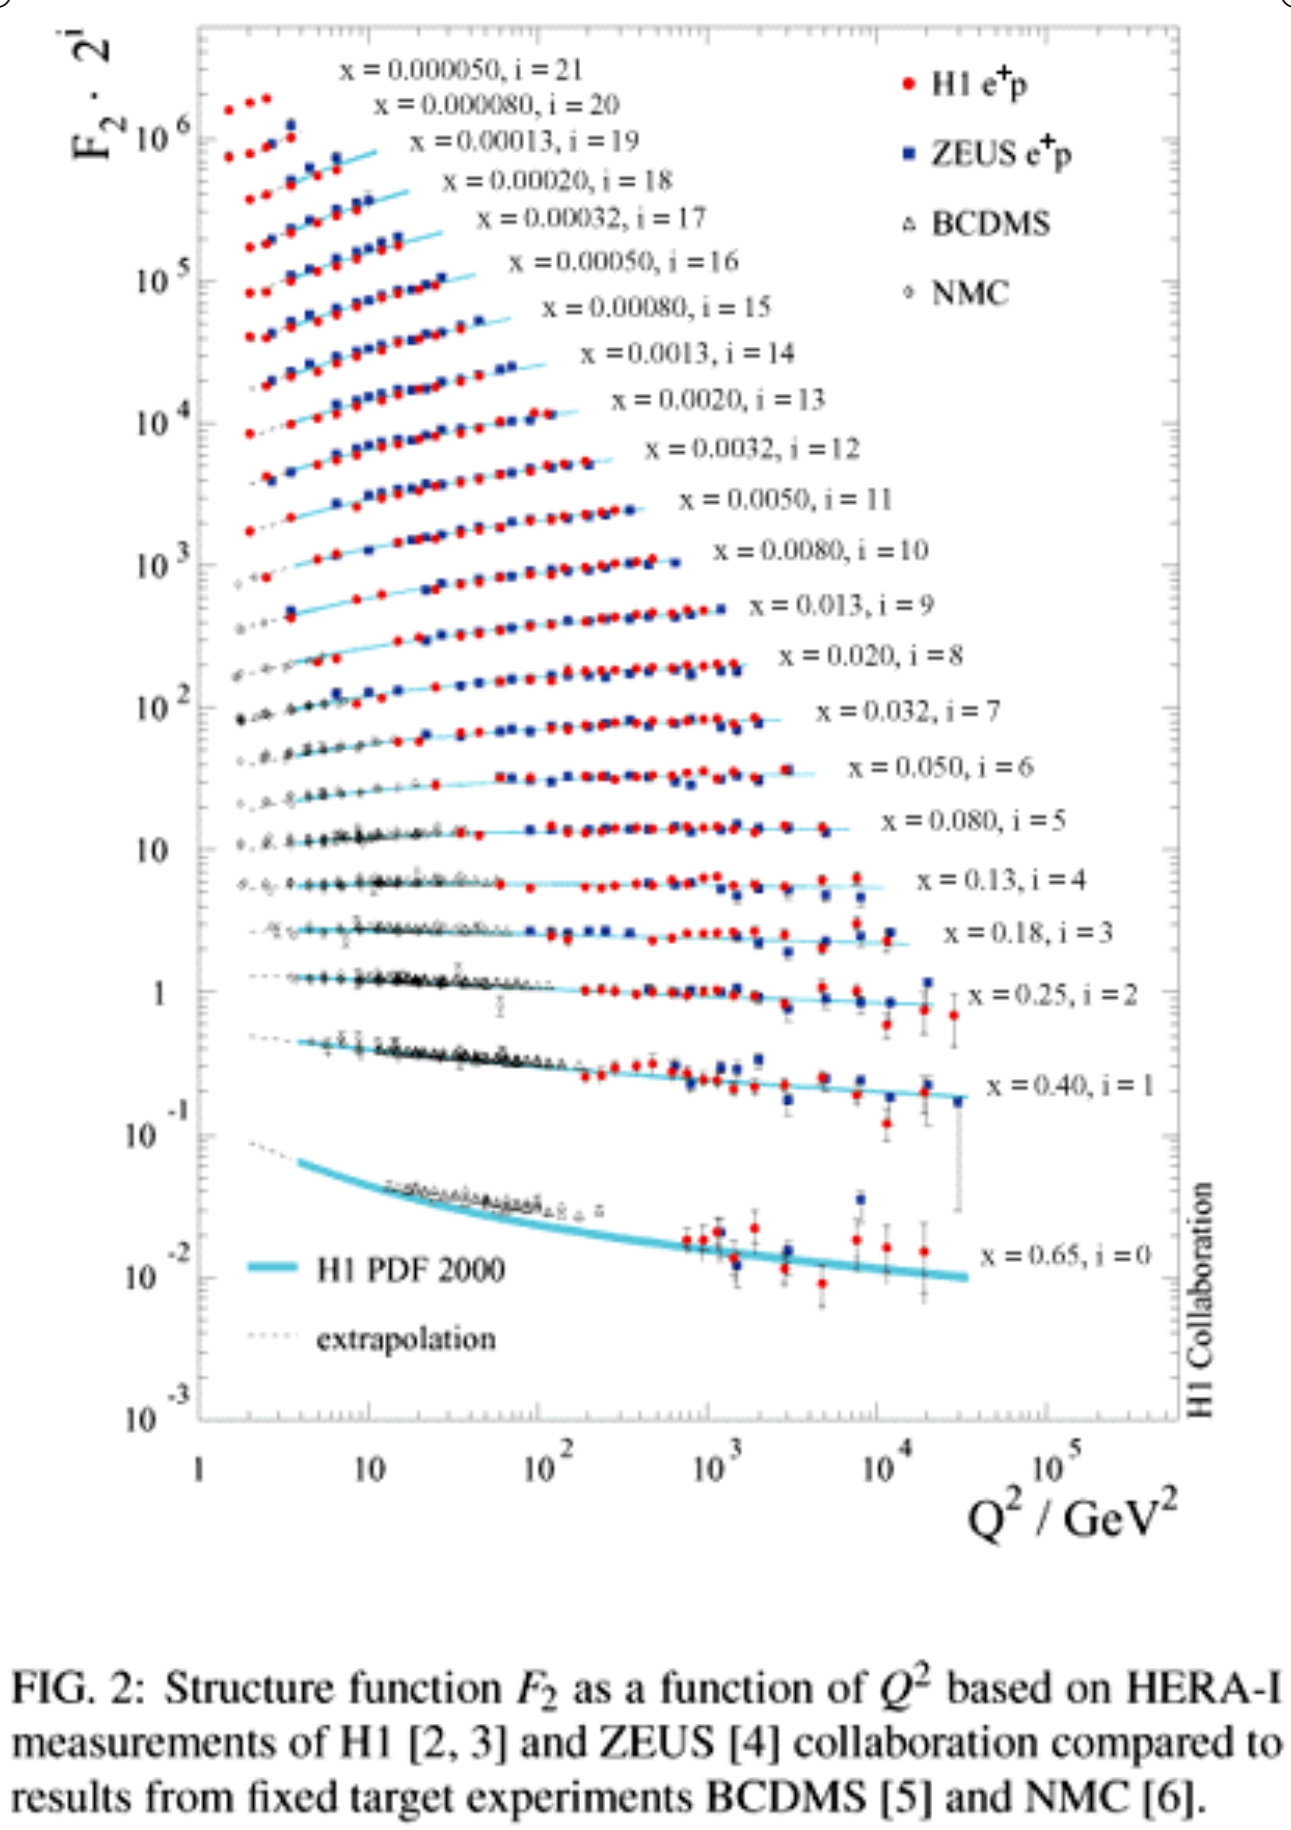
\includegraphics[width=10cm]{NuclearPhysics/modules/lepton-scattering/pics/inelastic-ep/Hera-dis.PNG}
            \caption{HERA structure functions}
        \end{figure}
        
        2 important takeaways:\\
        \newline
        1- Bjorken scaling holds up to $Q^2 = 20,000$ GeV$^2$, implying that quarks are point like up to scales of at least $10^{-18}$m. \\
        \newline
        2- \textbf{Scaling violations: }\\
        \newline
        \indent At medium X, we are independent of Q2, indicating we have quarks. At high x, the $F_2$ structure function decreases at high x, and increases at low x, with increasing $Q^2$. More specifically, imagine measuring the $F_2$ structure function across x at a certain $Q^2$. Now measure again at a higher $Q^2$. You will see the curve is shifted higher at low x, and lower at high x:
        
                
        \begin{figure}[H]
            \centering
            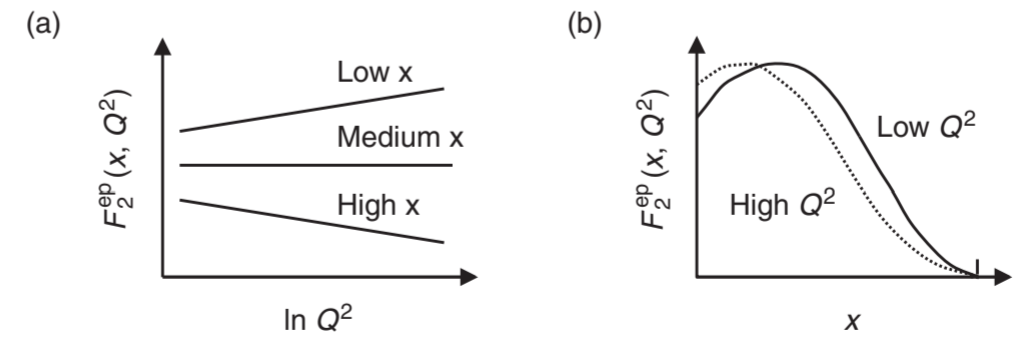
\includegraphics[width=12cm]{NuclearPhysics/modules/lepton-scattering/pics/inelastic-ep/scaling-violations.PNG}
            \caption{Explaination of Scaling Violations}
        \end{figure}
        
        This is indicative of the fact that at higher $Q^2$, the proton has a greater fraction of low x quarks. I.e., at low $Q^2$ we do not "see" the low-x quarks, but as we increase our resolving power, we do.\\
        \newline
        N.b. - we cannot measure the gluon PDFs, but can model them with QCD parton evolution equations such as DGLAP or BFKL.\\
        \newline
        Finally, we include a proton PDF at $Q^2$ = 10 GeV$^2$ and at $10^4$ GeV$^2$. (note - on a semilog plot!)
        
               
        \begin{figure}[H]
            \centering
            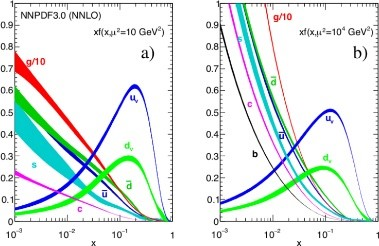
\includegraphics[width=14cm]{NuclearPhysics/modules/lepton-scattering/pics/inelastic-ep/PDFs.jpg}
            \caption{PDFs at two different $Q^2$ values}
        \end{figure}
     
 
